% 使用 XeLaTeX 编译。
\documentclass[UTF8,a4paper,11pt]{ctexart}
\usepackage[margin=24mm]{geometry}
\usepackage{graphicx}
\usepackage{amsmath,booktabs,xcolor}
\usepackage[colorlinks=true,linkcolor=blue]{hyperref}
\definecolor{ink}{HTML}{2463C7}
\ctexset{section/format=\Large\bfseries\color{ink}}
\newcommand{\methodname}{Source-first}
\title{LaTeX 工程教程}
\author{}
\date{}
\begin{document}
\maketitle
\begin{abstract}
本教程介绍 LaTeX 工程的文件结构、图片、公式和表格。该工程使用源码视图编辑，使用 PDF 视图查看排版。
\end{abstract}
\section{打开与编辑工程}
点击“打开”选择工程文件夹。切换到源码视图，通过文件列表打开各个源文件。
main.tex 是主文件，sections 目录存放章节。修改内容后按 Ctrl+S 保存，切换到 PDF 查看排版。

\section{插入图片}
图片文件保存在 figures 目录中。在 includegraphics 命令中设置 width 参数可调整宽度。例如，0.6\textbackslash linewidth 表示当前行宽的 60\%。
\begin{figure}[htbp]
  \centering
  % width 设置图片宽度。
  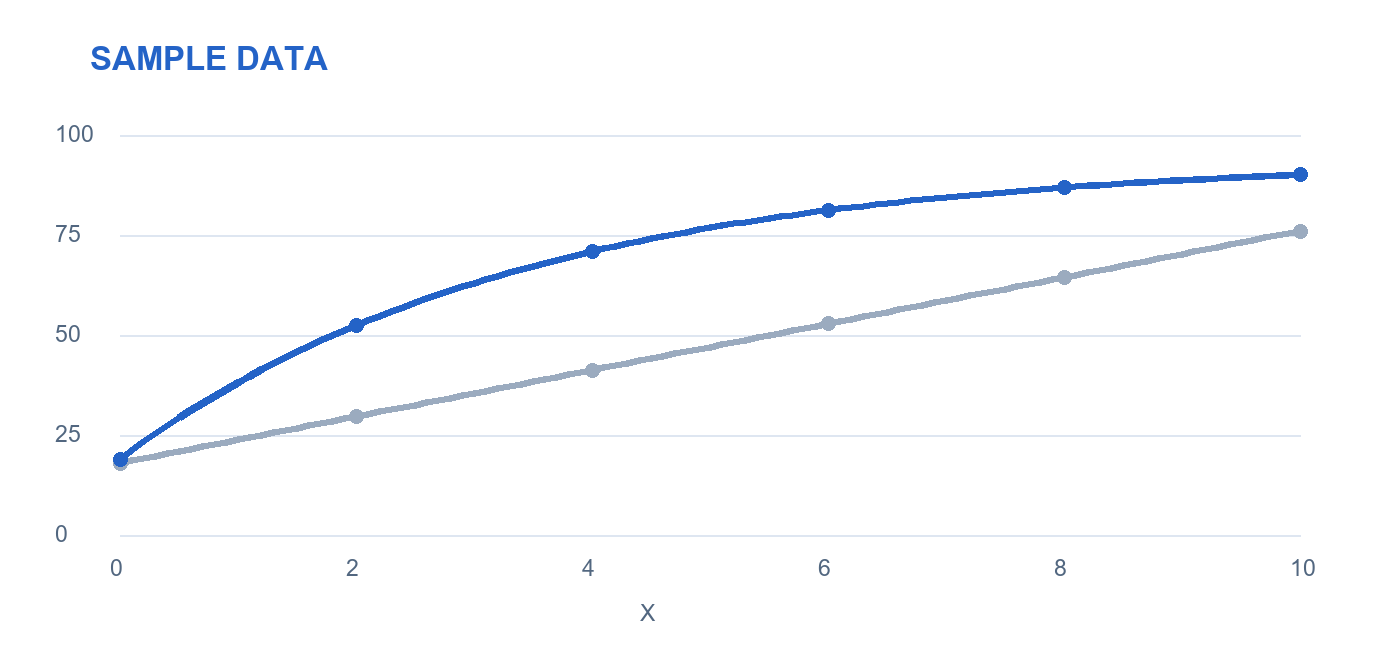
\includegraphics[width=0.6\linewidth]{figures/workflow.png}
  \caption{两组示例数据。}
  \label{fig:workflow}
\end{figure}
\section{公式与表格}
equation 环境用于独立公式，tabular 环境用于表格。
\begin{equation}
  a^2+b^2=c^2.
\end{equation}
\noindent 编译成功后，在 PDF 视图查看公式和表格。
\begin{center}
\begin{tabular}{ll}
\toprule
内容 & 命令或环境 \\
\midrule
图片 & includegraphics \\
独立公式 & equation \\
表格 & tabular \\
\bottomrule
\end{tabular}
\end{center}
\end{document}
